\documentclass{article}
\usepackage[preprint]{tmlr}
% PREPRINT MODE, for arXiv. [preprint] implies [accepted], so the author block
% below is printed. It also clears the running head and suppresses the "Reviewed
% on OpenReview" line, which is why \openreview stays at XXXXXX and is never
% consulted in this mode.
%
% TO GO BACK TO AN ANONYMOUS TMLR SUBMISSION: drop the option, so plain
% \usepackage{tmlr}, and comment the author block out again. Both, not one.
% Without the option the PDF is anonymous whatever the source says, but the
% source is not the PDF, and reviewers may be sent the project archive.

\usepackage{booktabs}
\usepackage{graphicx}
\usepackage{amsmath}
\usepackage{amssymb}
\usepackage{microtype}
\usepackage{url}

\title{Learned Heuristics Decay With Distance to Goal:\\
So Do Pattern Databases, by the Same Two-Moment Law}

% Live in preprint mode, ignored if the [preprint] option on line 2 is removed.
% Comment this back out whenever the anonymous submission build is rebuilt.
\author{\name Abhijoy Sarkar \email abhijoy.sar@gmail.com \\
        \addr Independent Researcher}

\def\month{08}
\def\year{2026}
\def\openreview{XXXXXX}

\begin{document}
\maketitle

\begin{abstract}
A heuristic is useful to a search only insofar as it orders the states that
search compares. \citet{wilt2016} measure this as Goal Distance Rank Correlation:
one Kendall $\tau$ against exact distance-to-goal, pooled over every pair. We
measure it \emph{stratified by distance} instead, against exhaustive ground
truth, on Rubik's-cube sub-problems from $5.5\times10^{2}$ to
$3.1\times10^{23}$ states and on sliding-tile boards.

Call the states at exact distance $d$ the \emph{shell} at $d$.
Search compares adjacent shells, and a heuristic's accuracy there is
$\Phi(\Delta/(\sigma\sqrt{2}))$, for $\Delta$ the gap in mean heuristic
value between shells and $\sigma$ the spread within them. Nothing is fitted.
On disjoint halves of each shell it gives mean absolute error $0.012$ over 252
observations against a noise floor of $0.002$, and it survives a
$300\times$ larger sub-problem, three further objectives, and injected noise.

Three consequences. Ordering quality is invariant to rescaling. Decay with
distance occurs exactly when $\sigma$ grows, so it is \emph{not} particular to
learned heuristics: pattern databases on the same states decay as much, in both
domains, and matched on strength the two classes are indistinguishable. And
$\sigma$ is the one term an objective can act on, yet every objective built to act on it
produced a worse heuristic.

The second domain bounds the law rather than confirming it. Error is four times larger on the
sliding tile, but that is not a fact about the state space:
the error tracks within-shell skewness, monotonically across three tasks, and
matched on skew the domains agree below $|\mathrm{skew}|=1$. The law is
skew-limited, not domain-limited.

We also show $\tau$-b rewards coarse-valued heuristics by enough ($0.084$) to
reverse comparisons it is used for. The identity is classical; the
measurement against exact ground truth is ours. We report three claims from
earlier versions that our own controls refuted.
\end{abstract}

\section{Introduction}

Learned heuristics for combinatorial search are usually judged by what a search
does with them: solve rate, solution length, nodes expanded. Each of those is a
property of the triple (heuristic, search algorithm, budget), not of the
heuristic. Change the beam width and every one of them moves. This makes them
poor instruments for the question practitioners actually face, which is whether a
trained heuristic is any good before committing compute to a search.

There is an established answer. \citet{chrestien2023} prove that forward search
with $f(s) = \alpha g(s) + \beta h(s)$ is strictly optimally efficient if and only
if $h$ is a perfect ranking, and conclude that ``the absolute value of the
heuristic is not important'', an observation credited to
\citet{xu2009} for beam search. \citet{wilt2016} turn this into a measurement:
Goal Distance Rank Correlation, Kendall's $\tau$ between $h$ and the exact
edge-count distance $d^*$, computed offline from a backward breadth-first search.
GDRC is search-independent, predicts greedy best-first expansions, and can be
optimised directly to construct heuristics.

Our starting point is that GDRC is a \emph{pooled} statistic, and that pooling
discards a structure the heuristics it summarises actually have: ordering quality
varies with distance from the goal. We expected that structure to be peculiar to
bootstrapped heuristics. Deep Approximate Value Iteration
\citep{agostinelli2019} anchors its value estimate at the goal and propagates
outward, so error should accumulate with distance by construction, and we
report that this expectation is wrong. Abstraction-based heuristics decay too,
and once heuristic strength is controlled the two classes are
indistinguishable. What survives is the measurement problem rather than the
mechanism story: a single coefficient averaged over all states cannot express a
distance-dependent profile, and is dominated by state pairs that are far apart,
which are easy to order and which no search ever compares.

\paragraph{Contributions.}
\begin{enumerate}\itemsep2pt
\item A family of Rubik's-cube sub-problems in which state-space cardinality can
be varied over 21 orders of magnitude with branching factor, encoding,
architecture and training budget held fixed, and in which \emph{depth can be
varied at exactly constant cardinality} by restricting the generating set
(Section~\ref{sec:setup}). Exhaustive ground truth is available on the small
rungs; a meet-in-the-middle prober, verified against that ground truth, extends
it by one further rung.
\item The measurement: ordering accuracy against exact ground truth, stratified
by true distance, and a strength-controlled comparison showing that the decay
it reveals belongs to informative heuristics in general, not to learned ones
(Section~\ref{sec:profile}). This is a negative result against our own initial
hypothesis, and Section~\ref{sec:profile} states plainly what the earlier,
under-controlled version of the comparison claimed.
\item A parameter-free account of that profile: per-shell ordering accuracy is
$\Phi(\Delta/(\sigma\sqrt{2}))$ in the between-shell gap and within-shell spread,
verified in and out of sample and across heuristic classes
(Section~\ref{sec:law}). It explains why the decay is universal, shows that
ranking quality is invariant to rescaling, and identifies within-shell spread as
the single term an objective can act on. We claim the measurement, not the
identity, which is standard signal detection theory.
\item A negative result on the intervention the law most obviously suggests
(Section~\ref{sec:losses}). Penalising within-shell spread is inert at low weight
and monotonically harmful at high weight, because it stalls the depth curriculum;
a ranking loss restricted to adjacent shells produces the flattest profile we
measured and one of the worst heuristics. Every objective that flattened the
profile degraded the search, which we report as a caution against reading the law
as a design target.
\item An exact decomposition of pooled $\tau$ into that profile, which makes the
dilution argument an identity rather than an intuition, and a measurement of a
bias in $\tau$-b that favours coarse-valued heuristics over continuous ones by
about $0.084$, enough to reverse comparisons of the kind this statistic is
routinely used for (Section~\ref{sec:pooled}).
\item Evidence that the pooled statistic is diluted by pairs search never makes,
including a run whose GDRC is indistinguishable from a working classical
heuristic while its adjacent-shell ordering is near chance
(Section~\ref{sec:pooled}).
\item A depth-versus-size experiment at constant cardinality, showing that size is
not the operative variable in that design, and, at ten seeds per condition,
that depth is not either over the range we can hold cardinality fixed
(Section~\ref{sec:depth}). A second correction lives here: the apparent failure
at the largest diameter, which an earlier version of this work reported as a
depth effect, is a curriculum-gate deadlock occurring in 1 run of 40 independently
of diameter. We give the one-integer diagnostic that distinguishes the two.
\end{enumerate}

\section{Background and related work}
\label{sec:related}

\paragraph{The nearest prior work.} \citet{wilt2016} define GDRC and validate it
as a predictor of search cost, reporting that ``when the GDRC is below roughly
0.4, greedy best-first search performs very poorly.'' Everything we might claim
about \emph{a ranking measure against exact ground truth} is theirs: it is
search-independent, ranking-based rather than magnitude-based, predictive, and
used prospectively to build heuristics. What remains is that GDRC is one scalar
per domain; their Algorithm~1 samples nodes from a backward BFS and returns a
single $\tau$. Our contribution is that same quantity resolved by distance. We
note that this is not only a correction applied to learned heuristics: the
pattern databases GDRC was designed around have distance-dependent profiles too
(Section~\ref{sec:profile}), so the pooling loss applies within its original
scope.

\paragraph{Predicting search cost is not new.} The Korf--Reid--Edelkamp formula
\citep{korf2001} predicts IDA* expansions from the heuristic's cumulative
\emph{value} distribution to within 1\% on Rubik's Cube. It is provably
ranking-blind: two heuristics with identical value histograms but different
state-to-value assignments receive identical predictions. It also constrains what
we may claim. KRE prove the asymptotic heuristic branching factor equals the
brute-force branching factor, so cost scales with problem growth; \emph{we
therefore make no claim that required search budget is independent of
state-space size}, and our depth experiment is designed only to rule size out
within a family where it is held constant.

\paragraph{Known failure modes, and how ours differs.}
\citet{hadar2026} diagnose train/deploy distributional shift in DAVI: search
oversamples low-heuristic states, causing systematic underestimation where search
operates. That is induced by the search's own sampling; our profile is measured on
states drawn independently of any search. \citet{hernandez2012} name ``heuristic
depression'', a \emph{bounded region} trapping real-time search; what we measure is
monotone in distance across the whole space. \citet{czechowski2021} quantify how a
learned value function's ordering degrades with the \emph{step spacing between
compared states} and report a signal-to-noise ratio at one fixed spacing, the
closest quantitative statement to ours, differing in the conditioning variable.
\citet{zawalski2024} observe qualitatively that value functions fail far from the
goal, but probe this by injecting distance-independent Gaussian noise, without
ground-truth comparison or stratification.

\paragraph{Scaling and capacity.} \citet{pendurkar2023} show the parameters needed
to approximate a heuristic grow exponentially in instance size and prove a
complexity-theoretic accuracy barrier. Their sweep varies instance size with
branching factor changing alongside; ours holds branching, encoding, architecture
and budget fixed. \citet{futuhi2026} publish ordinal value losses, PAC-dimension
bounds and \emph{near}-admissible learned heuristics with nonzero measured
overestimation. \citet{arfaee2011} bootstrap from backward random walks of
increasing length, which is the depth curriculum we adopt and claim nothing for.

\section{Experimental setup}
\label{sec:setup}

\paragraph{Notation.} Three terms recur. A \emph{shell} is the set of states at a
given exact distance from the goal; shell $d$ and shell $d+1$ are one move apart,
and those are the states a search compares against each other. A \emph{rung} is
one member of the family of sub-problems below, indexed by how many pieces it
tracks; higher rungs are exponentially larger. And $d^*(s)$ denotes the exact
number of moves from state $s$ to the goal, obtained by exhaustive search rather
than estimated. $\Phi$ is the standard normal distribution function throughout.

\paragraph{A ladder of sub-problems.} We track $k$ of the 24 edge ``wing'' pieces
of a $4\times4$ Rubik's cube and treat the remainder as interchangeable. This is
exactly the projection a pattern database uses, so each rung is a genuine
sub-problem: a move acts deterministically on the record of where the tracked
pieces are. Rung $k$ has $P(24,k) = 24!/(24-k)!$ reachable states, from 552 at
$k=2$ to $3.10\times10^{23}$ at $k=24$. Every rung uses the same 63 generators,
the same 24 slots and the same 600-wide one-hot encoding (24 slots $\times$ 25
symbols, the 25th being ``not tracked''), so only cardinality varies. Reachable
counts were verified against $P(24,k)$ by exhaustive search where feasible.

\paragraph{Exact ground truth.} Breadth-first search enumerates rungs to $k=6$
(96{,}909{,}120 states, 191\,MB, $\sim$22 minutes). Table~\ref{tab:exact} gives
the resulting diameters and mean distances. Diameter is exactly $k+2$
($R^2 = 1.00000$) and mean distance is $0.864k + 1.242$ ($R^2 = 0.99988$), so
across the ladder cardinality grows by 21 orders of magnitude while depth grows
linearly. Depth is therefore measured, not assumed, and cannot alone explain a
collapse of that shape.

\begin{table}[t]\centering\begin{tabular}{rrrr}
\toprule
$k$ & states & diameter & mean distance \\
\midrule
2 & 552 & 4 & 2.96 \\
3 & 12{,}144 & 5 & 3.83 \\
4 & 255{,}024 & 6 & 4.71 \\
5 & 5{,}100{,}480 & 7 & 5.58 \\
6 & 96{,}909{,}120 & 8 & 6.40 \\
\bottomrule
\end{tabular}
\caption{Exhaustive ground truth. Diameter is exactly $k+2$.}
\label{tab:exact}\end{table}

\paragraph{Beyond enumeration.} A meet-in-the-middle prober gives exact distances
for a \emph{sample} on larger rungs: build the ball of radius $f$ around the goal
once, then walk $b$ levels out from each query state and intersect. Before use it
is checked against exhaustive ground truth wherever both can run: 200/200
agreement at $k=4$ and 300/300 at $k=6$. It reaches one rung beyond enumeration
($k=8$); Section~\ref{sec:limits} explains why it stops there.

\paragraph{Varying depth at constant size.} Restricting the generating set leaves
the group generated unchanged (a half turn is two quarter turns), so the
reachable set is identical while the diameter grows. On rung $k=4$, four
generating sets all reach exactly 255{,}024 states (verified by exhaustive search)
at diameters 6, 8, 10 and 12. The cost of this design is that fewer generators
also means a smaller branching factor: it varies depth and branching together and
can rule out size, nothing more.

\paragraph{Training.} Deep Approximate Value Iteration \citep{agostinelli2019}
with a depth curriculum \citep{arfaee2011}: $J(s)=0$ if solved, else
$\min_a [1 + J_{\text{target}}(s')]$, with targets from a network frozen every 100
steps. Identical architecture (600--4096--2048--1024--1, 12.95M parameters),
batch 1024, Adam at $10^{-3}$, on every rung. Three seeds throughout; a seed sets
both the scramble stream and weight initialisation. Evaluation scrambles use a
separate fixed seed held constant across configurations, so any two checkpoints
are compared on identical states. Every solution is replayed on the puzzle before
being counted.

\paragraph{Sampling.} Profiles draw states across scramble lengths $1..16$ and
then \emph{measure} the true distance. Drawing from deep random walks (the
obvious choice, since it approximates the uniform distribution) concentrates
almost every state into the shells nearest the mean, leaving the shallow half of
the profile unmeasured. Scramble length is never used as the label: a state
scrambled nine moves is usually nearer than nine.

\section{Ordering accuracy decays with distance, for every informative
heuristic}
\label{sec:profile}

For each true-distance shell $d$ we measure
$\Pr[h(s) < h(s')]$ for $s$ at distance $d$ and $s'$ at $d+1$: can the heuristic
still tell closer from further? At $1.0$ it orders the two shells perfectly; at
$0.5$ it is a coin flip and search at that depth is blind, however small its
regression error.

\paragraph{The comparison, and the baseline that broke it.} We began by comparing
the DAVI-trained network against one pattern database (the exact distance
table of a smaller rung, admissible on the larger by abstraction) and a
uniform random control. On rung $k=6$ the learned heuristic decayed and the
abstraction was nearly flat, which we read as a signature of goal-anchored
bootstrapping. That reading does not survive a stronger baseline. The abstraction
we used was rung $k=2$, whose pooled GDRC on $k=6$ is $+0.570$; a heuristic that
weak is flat because it has little accuracy to lose, not because abstraction
confers distance-invariance. Table~\ref{tab:matched} reports every abstraction
available on that rung instead of one.

\begin{table}[t]\centering\begin{tabular}{lrrrr}
\toprule
heuristic & pooled GDRC & acc.\ at $d{=}1$ & at $d{=}6$ & decay \\
\midrule
random & +0.003 & 0.495 & 0.505 & -0.010 \\
PDB $k{=}$2 & +0.570 & 0.747 & 0.603 & +0.144 \\
PDB $k{=}$3 & +0.685 & 0.834 & 0.628 & +0.206 \\
PDB $k{=}$4 & +0.788 & 0.888 & 0.663 & +0.225 \\
\textbf{learned} & \textbf{+0.842} & \textbf{1.000} & \textbf{0.801} & \textbf{+0.199} \\
PDB $k{=}$5 & +0.891 & 0.990 & 0.712 & +0.278 \\
\bottomrule
\end{tabular}
\caption{Rung $k=6$, all heuristics on identical states and identical exhaustive
ground truth, ordered by pooled GDRC. Decay grows with strength across the
column, and the steepest decay belongs to a pattern database, not to the learned
heuristic.}
\label{tab:matched}\end{table}

\begin{figure}[t]\centering
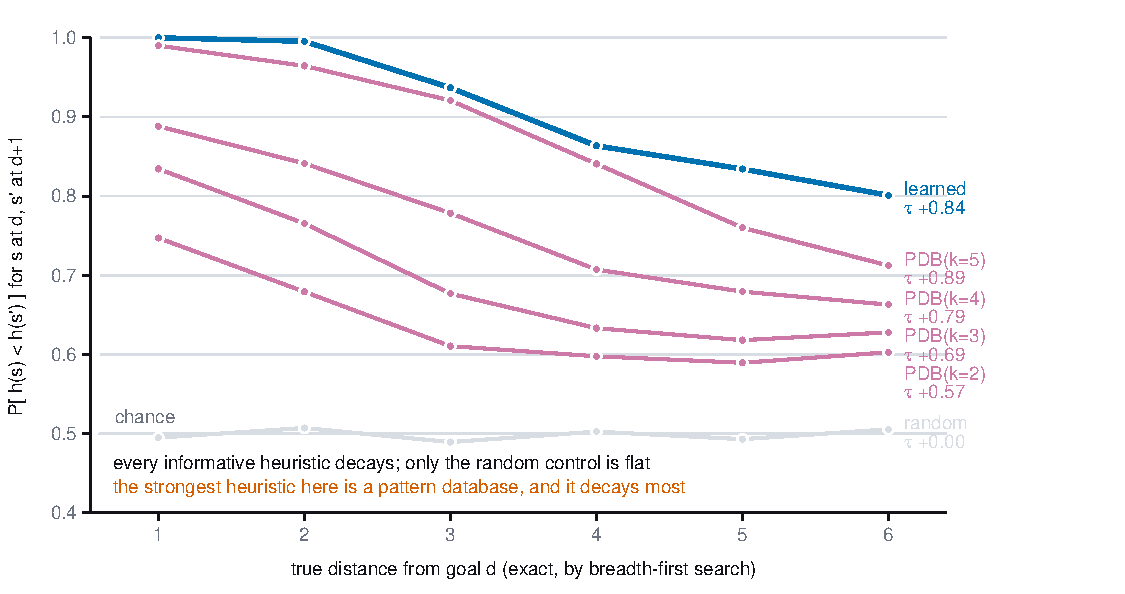
\includegraphics[width=0.86\linewidth]{figures/fig13.pdf}
\caption{Ordering accuracy by true distance on rung $k=6$. Every informative
heuristic is near-perfect adjacent to the goal and decays outward; only the
random control is flat. Showing PDB($k{=}2$) alone, the lowest curve above
chance, is what made the decay look particular to the learned heuristic.}
\label{fig:profile}\end{figure}

\paragraph{Controlling for strength.} Decay is a function of how good a heuristic
is. Across 39 distinct heuristics (22 learned checkpoints, 12 abstractions, 5
random controls) it correlates with pooled GDRC at $r = +0.588$
($p = 8.3\times10^{-5}$; Figure~\ref{fig:strength}). Regressing decay on GDRC and
comparing residuals, learned heuristics sit $+0.006$ above the fit and
abstractions $-0.016$ below it, a difference of $+0.023$ that is not detectable
(Welch $t = +0.72$, $p = 0.48$) and whose 95\% confidence interval,
$[-0.039,+0.084]$, is small relative to the mean decay of $0.154$. The strictest
form of the test matches each learned heuristic to the abstraction nearest it in
GDRC \emph{on the same sampled states} (median gap $0.057$): across 18 such pairs
the abstraction decays more in 13, and the two mean decays agree to three
decimals at $+0.154$.

\begin{figure}[t]\centering
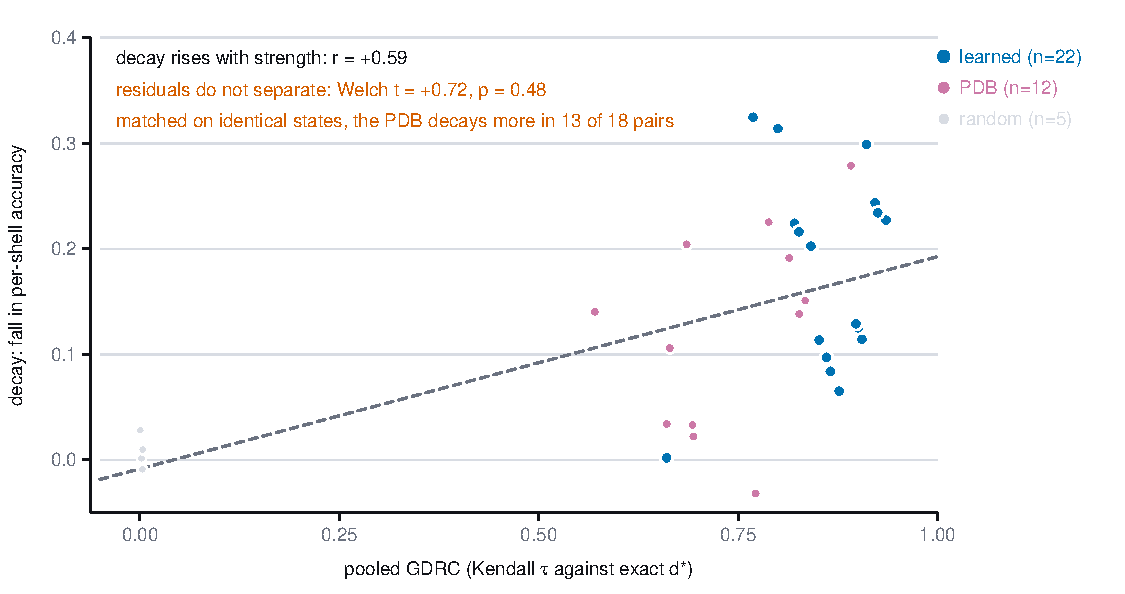
\includegraphics[width=0.86\linewidth]{figures/fig14.pdf}
\caption{Decay against pooled GDRC for every distinct heuristic measured. The
dashed line is the least-squares fit. Learned points do not sit above it. Repeats
are collapsed: a profile is written per learned checkpoint and re-measures the
same abstractions on the same states, so counting each appearance separately
would inflate $n$ from 39 to 98.}
\label{fig:strength}\end{figure}

\begin{table}[t]\centering\begin{tabular}{lrrr}
\toprule
heuristic class & $n$ & mean GDRC & mean decay \\
\midrule
random & 5 & +0.003 & +0.003\,$\pm$\,0.014 \\
PDB & 12 & +0.741 & +0.125\,$\pm$\,0.095 \\
learned & 22 & +0.860 & +0.171\,$\pm$\,0.085 \\
\midrule
\multicolumn{4}{l}{decay vs.\ strength: $r = +0.594$ over 39 observations ($p = 6.7\!\times\!10^{-5}$)} \\
\multicolumn{4}{l}{residual about that fit: learned $+0.0062$, PDB $-0.0162$; Welch $t = +0.72$, $p = 0.48$} \\
\multicolumn{4}{l}{\quad difference $+0.0224$, 95\% CI $[-0.039, +0.084]$} \\
\multicolumn{4}{l}{matched on identical states: PDB decays more in 13 of 18 pairs} \\
\bottomrule
\end{tabular}
\caption{The strength control in full.}
\label{tab:strength}\end{table}

\paragraph{What does survive.} The profile itself, and its dependence on depth.
The decay grows with diameter at \emph{constant} cardinality of 255{,}024 states:
$0.108 \pm 0.008$ at diameter 6, $0.123 \pm 0.006$ at 8, and $0.259 \pm 0.029$ at
10 (mean over three seeds). On rung $k=8$ ($2.97\times10^{10}$ states), where
ground truth comes from the verified prober, learned accuracy runs $1.000$ at
$d=1$ to $0.677$ at $d=6$. So there is a real distance-dependent structure to
measure, in a heuristic class where it was expected and in one where it was not,
and Section~\ref{sec:pooled} is about the fact that a pooled coefficient reports
none of it.

\paragraph{What we no longer claim.} That the profile distinguishes learned
heuristics from classical ones, or that its shape diagnoses bootstrapping. We
report the earlier claim and its refutation rather than deleting it, because the
error is instructive: the flat baseline was not evidence of a mechanism, it was
an artifact of comparing against something barely better than chance.

\section{The profile is a two-moment quantity}
\label{sec:law}

Section~\ref{sec:profile} leaves the decay described but unexplained. The
explanation is one sentence: a heuristic tells two shells apart exactly as well as
the gap between their average values is large compared with the scatter of values
inside them. If the averages differ by one move and values scatter by a tenth of a
move, the two shells barely overlap and ordering is near-perfect; if they scatter
by a full move, the shells overlap heavily and ordering approaches a coin flip.
Nothing about the heuristic's provenance enters. Formally: Write $\mu(d)$
for the mean heuristic value on shell $d$, $\sigma(d)$ for the within-shell
spread, and
\[
  \Delta(d) = \mu(d{+}1) - \mu(d), \qquad
  d'(d) = \frac{\Delta(d)}{\sqrt{\tfrac{1}{2}\left(\sigma(d)^2 + \sigma(d{+}1)^2\right)}} .
\]
If the two shells' value distributions were normal with equal variance, the
probability that a draw from the nearer shell falls below a draw from the further
one would be exactly $\Phi(d'/\sqrt{2})$. We find that this predicts the measured
ordering accuracy across our data:
\begin{equation}
  a(d) \;=\; \Phi\!\left(\frac{d'(d)}{\sqrt{2}}\right).
  \label{eq:law}
\end{equation}
Nothing here is fitted. There is no coefficient, no intercept, and no per-domain
constant, so Equation~\ref{eq:law} is a prediction that could simply be wrong,
most obviously for pattern databases, whose values are small integers with heavy
ties and no reason whatever to look normal.

\begin{table}[t]\centering\begin{tabular}{lrrrr}
\toprule
sample & $n$ & mean $|$error$|$ & noise floor & max $|$error$|$ \\
\midrule
exhaustive ground truth, $k\!\le\!6$ & 252 & 0.0117 & 0.0018 & 0.081 \\
\quad \emph{same, moments and accuracy from one sample} & 252 & 0.0087 & 0.0018 & 0.050 \\
\midrule
\emph{held out}: probed ground truth, $k\!=\!8$ & 6 & 0.0078 & 0.0024 & 0.017 \\
\emph{held out}: other training objectives & 152 & 0.0147 & 0.0022 & 0.094 \\
\midrule
\multicolumn{5}{l}{Two free parameters, $\Phi(d'/s + b)$, give mean $|$error$|$ 0.0082 at $s = 1.451$,} \\
\multicolumn{5}{l}{\quad against 0.0087 at the parameter-free $s = \sqrt{2} = 1.414$} \\
\bottomrule
\end{tabular}
\caption{Equation~\ref{eq:law} against measurement. Each observation is one
heuristic at one true-distance shell.}
\label{tab:law}\end{table}

\begin{figure}[t]\centering
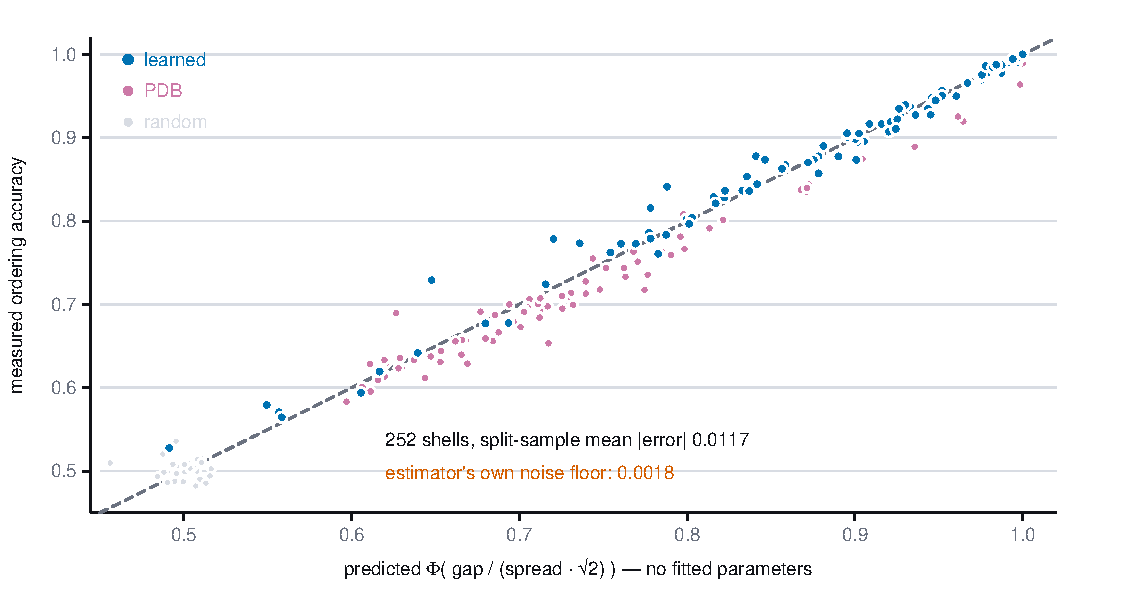
\includegraphics[width=0.82\linewidth]{figures/fig15.pdf}
\caption{Predicted against measured ordering accuracy; the dashed line is
$y = x$. Pattern databases sit slightly below it, which is the cost of their
discreteness, the one place the normal approximation is visibly imperfect.}
\label{fig:law}\end{figure}

\paragraph{The estimate must not use the states it is scored on.} Accuracy and
the two moments are both computable from the same sampled shell, and if they are,
the comparison is partly circular: a shell whose sampled mean happens to sit high
yields both a higher predicted accuracy and a higher measured one. The size of
that effect is not small. Run this estimator on a heuristic with \emph{no signal
at all} and it reports a correlation of $+0.95$ between prediction and
measurement where the truth is zero. We therefore split every shell, estimate
$\Delta$ and $\sigma$ on one half and measure accuracy on the other, and report
the split figures throughout. The correlations survive for informative
heuristics and collapse for the random control, which is the expected signature,
and is why we do not quote a correlation coefficient as evidence anywhere in
this paper.

Table~\ref{tab:law} and Figure~\ref{fig:law} report the comparison. Split-sample,
the mean absolute error is $0.012$ over 252 shell observations. That is roughly
six times the noise floor of the estimator itself ($0.002$, from the binomial
error of accuracies computed on 20{,}000 sampled pairs), so the residual is real
structure rather than measurement noise: the law is a good approximation, not
an exact one. It holds on rung $k=8$, where ground truth comes from the
meet-in-the-middle prober rather than exhaustive search ($0.008$), and on 152
shell observations from heuristics trained under three objectives introduced
after this measurement was designed ($0.015$). The error is largest for pattern
databases, whose small-integer values are the furthest from normal.

\paragraph{Is the form right, or merely monotone?} Any increasing function of
$d'$ would track the measurement, so agreement alone is not the test. Granting
the model two free parameters, $\Phi(d'/s + b)$, improves the mean absolute error
only from $0.0087$ to $0.0082$, at $s = 1.451$ against the $\sqrt{2} = 1.414$ the
identity specifies. A fitted logistic does worse ($0.010$). We note that $\sqrt{2}$
is not an empirical discovery: it appears because we write the denominator as a
root-mean-square of the two shells' spreads, and
$\Phi(\Delta/(\sigma_{\mathrm{rms}}\sqrt{2}))$ is identically
$\Phi(\Delta/\sqrt{\sigma_1^2+\sigma_2^2})$, which is exact for independent
normals. What the fit tests is whether real value distributions behave like that,
and they do, to within about 3\% in the effective scale.

\paragraph{Breaking it on purpose.} Everything above is observational: we
measured heuristics that happened to exist. That leaves two objections. The
comparison could be confounded, since our heuristics differ in rung, diameter,
network and training. And it could be vacuous, since any increasing function of
$d'$ would track the measurement.

Both are answerable by manufacturing heuristics with known perturbations. Take a
trained network and add deterministic per-state noise,
$h_\lambda(s) = h(s) + \lambda\,\varepsilon(s)$, with $\varepsilon$ derived by
hashing the state's index so that $h_\lambda$ remains a function of the state.
Every point in the sweep then shares rung, diameter, network and training exactly,
which disposes of the first objection. The second is settled by the choice of
noise family, because Equation~\ref{eq:law} has no right to work when the
perturbation has no variance to speak of.

\begin{table}[t]\centering\begin{tabular}{llrrr}
\toprule
noise family & tails & $n$ & measured & forward \\
\midrule
uniform & lighter than normal & 6 & 0.0042 & 0.0065 \\
gaussian & normal (the assumption) & 6 & 0.0046 & 0.0079 \\
laplace & heavier, finite variance & 6 & 0.0123 & 0.0458 \\
\textbf{cauchy} & \textbf{no finite variance} & 6 & \textbf{0.1654} & \emph{undefined} \\
\midrule
\multicolumn{5}{l}{Mean absolute error of Equation~\ref{eq:law}, over $\lambda \in \{0.25, 0.5, 1.0, 2.0, 4.0, 8.0\}$ in units of the} \\
\multicolumn{5}{l}{unperturbed within-shell spread. \emph{Forward} uses only the $\lambda\!=\!0$ moments.} \\
\bottomrule
\end{tabular}
\caption{Injecting calibrated noise into a trained heuristic on rung $k=6$.
\emph{Measured} recomputes both moments from the perturbed heuristic;
\emph{forward} predicts accuracy from the unperturbed moments plus the analytic
variance inflation $\lambda^2\mathrm{Var}(\varepsilon)$, touching the perturbed
heuristic only to score it.}
\label{tab:noise}\end{table}

Table~\ref{tab:noise} reports the outcome, and it is the sharpest evidence in
this paper. The error grows monotonically with the tail weight of the injected
noise: uniform and Gaussian noise leave the prediction intact
($0.004$--$0.005$), Laplace noise degrades it about threefold, and Cauchy noise,
which has no finite variance, breaks it by a factor of $36$, to $0.165$.
A law that were merely monotone in $d'$ would have no reason to care which
distribution the noise came from. This one does, in the direction and roughly the
proportion the normal approximation implies.

The \emph{forward} column is the causal test. Adding independent noise of
variance $v$ inflates each shell's variance by exactly $\lambda^2 v$ and leaves
the gap alone, so the unperturbed moments alone predict the perturbed accuracy
with nothing fitted and nothing measured on the perturbed heuristic. That
prediction holds to $0.008$ on average and $0.013$ at $\lambda = 8$, where the
injected noise is eight times the heuristic's own within-shell spread. For Cauchy
the forward prediction cannot even be written down, which is the same fact
stated twice.

\paragraph{Three consequences.} First, $d'$ is a ratio, so it is invariant to
rescaling: multiplying a heuristic by a constant moves $\Delta$ and $\sigma$
together and leaves $a(d)$ untouched. No amount of recalibrating output
magnitudes can improve ranking, which also disposes of the span-based diagnostic
we withdrew in Section~\ref{sec:pooled}. Second, the decay of
Section~\ref{sec:profile} is not a consequence of a heuristic being good or bad:
holding $\sigma$ constant across shells makes $a(d)$ constant and the decay
exactly zero, whatever the overall accuracy. Ordering quality falls with distance
if and only if within-shell spread grows with distance, and it does for every
heuristic we measured. But it does so in strikingly different ways, and an
earlier version of this work got that wrong: pooling all heuristics gave
$\sigma(d) \approx \sigma_0(1+0.21\,d)$, which we reported as a property of the
state space. Separated by class, the two do not resemble each other at all.
Abstractions grow gently from a wide base ($\beta = 0.15$, $\sigma_0 = 0.40$,
$n=11$); learned networks grow steeply from a narrow one ($\beta = 2.04$,
$\sigma_0 = 0.04$, $n=21$), with no overlap in range. The pooled figure was the
abstraction value, surfacing because duplicated rows gave abstractions three
times their true weight.

The corrected statement is more interesting than the one it replaces. The two
classes arrive at comparable decay from opposite directions: a pattern database
starts imprecise and degrades slowly, a learned network starts sharp and degrades
fast, which is why matching them on overall strength makes their decay
indistinguishable while their mechanisms are not.

Third, and most usefully, adjacent shells are one move apart, so $\Delta$ is
pinned near $1$ for any heuristic calibrated to distance; we measure $0.917$
for learned heuristics and $0.600$ for abstractions, whose values compress
because abstraction shortens distances. The only remaining free term is
$\sigma$. A squared-error objective charges bias and variance alike; ordering is
indifferent to bias and cares only about variance relative to a gap it cannot
enlarge. Section~\ref{sec:losses} tests whether an objective that targets that
term directly yields a better heuristic. It does not, and the way it fails is
itself informative.

\paragraph{What this is and is not.} Equation~\ref{eq:law} is not new and we
claim no part of it. It is the equal-variance binormal identity relating $d'$ to
the area under an ROC curve \citep{hanley1982}, which descends from
\citet{thurstone1927}; the observation that per-shell ordering accuracy is a
pairwise-class decomposition of AUC is \citet{hand2001}. Nearest in our own
setting, \citet{czechowski2021} model a learned value function as
distance-plus-Gaussian-noise and report ordering-inversion rates against step
separation, which is the same mechanism argued from the same premise. What we report is that it holds, parameter-free
and to about one percentage point, for heuristic ordering quality measured
against exact ground truth, across learned networks, integer-valued pattern
databases and random controls, on every rung and diameter we can measure. Its
value is that it reduces a profile to two interpretable numbers and identifies
which of them an intervention can move.

\section{Trying to flatten the profile makes the heuristic worse}
\label{sec:losses}

Section~\ref{sec:law} identifies within-shell spread as the term an objective can
act on. We tried to act on it, and report the outcome in full because it is
negative in an informative way.

\begin{table}[t]\centering\begin{tabular}{lrrrr}
\toprule
objective & solve rate & decay & beam width & curriculum \\
\midrule
\textbf{squared error (baseline)} & \textbf{100.0\%} & \textbf{0.219} & \textbf{24.0} & \textbf{40} \\
pairwise rank, uniform pairs & 59.8\% & 0.354 & 302.2 & 33 \\
pairwise rank, adjacent pairs only & 44.3\% & 0.145 & 131.3 & 37 \\
\midrule
\quad $+$ variance penalty, $\lambda=1$ & 100.0\% & 0.223 & 21.8 & 40 \\
\quad $\lambda=3$ & 100.0\% & 0.247 & 18.3 & 25 \\
\quad $\lambda=10$ & 99.5\% & 0.417 & 49.2 & 7 \\
\quad $\lambda=30$ & 92.0\% & 0.471 & 79.2 & 10 \\
\bottomrule
\end{tabular}
\caption{Four training objectives on rung $k=6$, identical in architecture,
budget, seeds and curriculum criterion. Beam width is the smallest reaching a
90\% solve rate; ``curriculum'' is the scramble depth the run reached, out of 40.
Three seeds each; runs that never left the first curriculum level are excluded.}
\label{tab:losses}\end{table}

We compare squared error against a RankNet-style pairwise logistic, the same loss
restricted to pairs one shell apart, and squared error plus an explicit
within-shell variance penalty at four weights. All arms share a scale-invariant
curriculum criterion, because the default criterion advances on squared error and
a scale-free ranking loss can never satisfy it, and using it would have pinned
those arms at the first level and manufactured the result.

\paragraph{Nothing beat the baseline.} At $\lambda = 1$ the variance penalty is
indistinguishable from squared error on every measure (decay $0.223$ against
$0.219$, $p = 0.77$; beam width $21.8$ against $24.0$, $p = 0.70$). Both ranking
arms are substantially worse, and both are unstable: their outputs are
scale-free, and across seeds the range of network outputs spanned $16$ to $2817$.

\paragraph{Pushing harder makes it worse, monotonically, and we can see why.}
Raising the penalty weight moves the decay in the wrong direction with perfect
rank consistency ($\rho = +1.00$ across $\lambda \in \{0,1,3,10,30\}$), and the
mechanism is visible in the last column of Table~\ref{tab:losses}: the curriculum
level reached falls with $\lambda$ ($\rho = -0.87$). Penalising within-shell
spread makes the network's outputs more nearly constant, a curriculum gated on
adjacent-shell separation reads that as failure to learn the current level, and
the run never reaches the depths whose ordering the penalty was meant to protect.
At $\lambda = 10$ training stalls at scramble depth 7 of 40.

\paragraph{The flattest profile belongs to the worst heuristic.} The
adjacent-pairs ranking loss produces exactly the effect
Section~\ref{sec:law} predicts. Restricted to the comparisons a search
actually makes, it yields the flattest profile we measured, decay $0.145$ against
the baseline's $0.219$, it solves 44\% of scrambles against the baseline's
100\%. Every arm here that succeeded in flattening the profile also degraded the
heuristic, and the two effects are not separable in our data.

\paragraph{What we take from this.} The decay is not a defect waiting to be
removed. Within-shell spread is not noise contaminating a signal: it is how a
heuristic distributes its predictions over depth at all, and suppressing it
suppresses the thing being measured. A reader who takes Equation~\ref{eq:law} as
a design target should read this section first. We do not claim the space of
interventions is exhausted, since targeting the numerator, or the variance of the
bootstrap target rather than of the network, remain untried, only that the
most direct reading of the law does not work, and fails for a reason the law
itself does not anticipate.

\section{What a pooled coefficient hides}
\label{sec:pooled}

The dilution can be stated exactly rather than argued. Pairs tied in $d^*$ are
precisely the pairs drawn from the same shell, so with $n_s$ sampled states at
distance $s$ and $a(s,t)$ the probability that $h$ ranks a state at $s$ below one
at $t$,
\[
  C - D \;=\; \sum_{s<t} n_s n_t \bigl(2\,a(s,t) - 1\bigr),
  \qquad
  n_0 - n_1 \;=\; \sum_{s<t} n_s n_t ,
\]
so $\tau$ is an $n_s n_t$-weighted average of ordering accuracy over \emph{every}
pair of shells. Adjacent shells are a vanishing share of that sum. A search never
makes the other comparisons: beam search, greedy best-first and A* all compare a
node against its siblings, one move apart and therefore in adjacent shells.
\textbf{The comparison a search depends on is the hardest one, and it is the one
$\tau$ dilutes most.} Combining this identity with Equation~\ref{eq:law}, which
supplies $a(s,t)$, predicts the pooled coefficient from the profile alone to
within $0.016$ for learned heuristics, so the profile, not the scalar, is the
more fundamental object.

One run of the forty in Section~\ref{sec:depth} degenerated: the deadlocked
one, which trained only within two moves of the goal. It is used here as a case
study in what a pooled coefficient conceals, not as evidence about depth. Its
pooled $\tau$ is $+0.660$, comparable to the abstractions available on those same
states (PDB $k{=}2$ at $+0.693$, PDB $k{=}3$ at $+0.772$) and far below its
sibling seeds at $+0.936$. Those PDB figures are inflated by ties: corrected as in
the next paragraph, PDB $k{=}2$ scores $+0.618$, so a pooled $\tau$ ranks
this crippled network \emph{above} a working pattern database. Its per-shell profile shows why:
adjacent-shell accuracy falls to $0.498$ by $d=9$ while the pooled coefficient
stays near $+0.66$, because that coefficient is dominated by the far-apart pairs
the identity above weights most heavily. It orders distant states well and
adjacent ones barely above chance; $\tau$ reports the average, while search
experiences only the adjacent column.

\paragraph{$\tau$-b also rewards a heuristic for being coarse.} Kendall's
$\tau$-b divides by $\sqrt{(n_0-n_1)(n_0-n_2)}$, where $n_1$ counts pairs tied in
the heuristic. A heuristic with no ties is charged for its arbitrary
\emph{within}-shell ordering, and one that ties inside each shell is not. On our
$k=6$ sample a tie-free heuristic that orders every shell perfectly is capped at
$0.919$, while the exact distance function, which makes the identical shell
ordering but is integer-valued, scores $1.000$. Both are computed
analytically and checked against \texttt{scipy}, which agrees to four decimals.

The gap is not a curiosity. Pattern databases are small integers; learned
heuristics are continuous. Breaking each abstraction's ties at random, which
leaves its between-shell ordering completely unchanged, costs it $0.070$ to
$0.101$ of pooled $\tau$ across our configurations (mean $0.084$). That is the
same magnitude as the differences the learned-versus-classical literature
reports from this statistic. Comparing the two classes by GDRC is therefore not a
like-for-like comparison. That $\tau$-b is sensitive to ties is
\citet{kendall1945}'s own observation and not a new one; what appears not to have
been noted is that it is large enough to reverse the learned-versus-classical
comparisons this statistic is used to make in search. The remedy is one line:
break ties at random before correlating, report $\tau$ both ways, or use an
asymmetric measure such as \citet{somers1962}'s $D$, which conditions on the
variable that has the ties.

\paragraph{A correction.} We first attributed this to $\tau$ being
scale-invariant, since that run's outputs span only $0.004$. That explanation is
wrong: a heuristic with a small span and clean ordering works perfectly well, and
\citet{wilt2016} rely on scale-invariance deliberately. What degrades the run is
that its within-shell spread ($\approx 6\times10^{-4}$) exceeds its between-shell
gap ($\approx 2\times10^{-4}$), so adjacent shells overlap. Span is not a
diagnostic and we do not propose it as one.

\paragraph{Solve rate is not a substitute.} That same degenerate run still solved
73.5\% of its evaluation scrambles. With 12 generators at beam width 100 over
depth 60, the search touches an appreciable fraction of a 255{,}024-state space:
this is beam search brute-forcing the problem, not the heuristic contributing.

\section{Neither depth nor size, in this range}
\label{sec:depth}

\begin{table}[t]\centering\begin{tabular}{lrrrrr}
\toprule
generators & \#moves & diameter & seeds & solve rate & excl.\ deadlocked \\
\midrule
\texttt{all} & 63 & 6 & 10 & 100.0\,$\pm$\,0.0 & -- \\
\texttt{oi-q} & 24 & 8 & 10 & 100.0\,$\pm$\,0.0 & -- \\
\texttt{oi-q4} & 16 & 10 & 10 & 100.0\,$\pm$\,0.0 & -- \\
\texttt{oi-q3} & 12 & 12 & 10 & 97.3\,$\pm$\,8.0 & 100.0\,$\pm$\,0.0 \\
\midrule
\multicolumn{6}{l}{1 of 40 runs never advanced past the first curriculum level; see Section~\ref{sec:depth}} \\
\bottomrule
\end{tabular}
\caption{Rung $k=4$ at four generating sets. Every row has exactly 255{,}024
reachable states, verified by exhaustive search; only the diameter differs. Ten
seeds each, identical 12{,}000-step budget.}
\label{tab:depth}\end{table}

Table~\ref{tab:depth} holds cardinality exactly constant and varies only the
generating set. Doubling the diameter from 6 to 12 changes the solve rate by
nothing measurable: every seed at every diameter solves every evaluation
scramble, with the single exception discussed below. Cardinality is ruled out by
construction, and depth is not doing anything either over this range.

\paragraph{A correction, and how we found it.} An earlier version of this section
reported that performance ``breaks at diameter 12'', on the strength of three
seeds of which one collapsed. Checking the final curriculum level of every
checkpoint showed that the collapsed run had never left the first level: its
network settled to a constant at scramble depth 2, its squared error therefore
never fell below the threshold that advances the curriculum, and it spent all
12{,}000 steps training on states within two moves of the goal. It did not fail
at depth; it never trained at depth. Re-running the experiment at ten seeds per
diameter puts that failure rate at 1 in 40, and the failure is not associated
with diameter (1 of 10 at diameter 12 against 0 of 30 elsewhere, Fisher exact
$p = 0.25$). With that run removed, every cell in the table is
$100.0 \pm 0.0$.

We report this because the failure mode generalises past our own experiment. A
curriculum gated on a loss threshold is a feedback loop: a run that fails to fit
the current level is denied the deeper data that might have dislodged it. The
resulting collapse looks exactly like a hard instance (low solve rate, tiny
output range, near-chance ordering far from the goal) and is nothing of the
kind. The diagnostic is one integer, the curriculum level reached, and it costs
nothing to record.

\paragraph{What we still claim here.} That state-space cardinality is not the
operative variable, which the design establishes by holding it exactly constant.
Not that depth is: this range shows no depth effect at all, and a design that
varies depth and branching factor together could not have attributed one anyway.
Seed variance across the \emph{size} ladder (Table~\ref{tab:ladder}) is a
separate matter and is unaffected, because every run there reached the curriculum
ceiling, so its $\pm23.5$ percentage points at $k=10$ is genuine variation rather
than this deadlock.

\begin{table}[t]\centering\begin{tabular}{rrrrr}
\toprule
$k$ & states & \multicolumn{3}{c}{solve rate at training budget} \\
\cmidrule(l){3-5}
 & & 3k & 12k & 40k \\
\midrule
2 & $5.52\!\times\!10^{2}$ & 100.0\,$\pm$\,0.0 & 100.0\,$\pm$\,0.0 & 100.0\,$\pm$\,0.0 \\
4 & $2.55\!\times\!10^{5}$ & 100.0\,$\pm$\,0.0 & 100.0\,$\pm$\,0.0 & 100.0\,$\pm$\,0.0 \\
6 & $9.69\!\times\!10^{7}$ & 93.5\,$\pm$\,5.8 & 100.0\,$\pm$\,0.0 & 99.8\,$\pm$\,0.2 \\
8 & $2.97\!\times\!10^{10}$ & 16.3\,$\pm$\,14.4 & 81.3\,$\pm$\,7.0 & 93.3\,$\pm$\,4.9 \\
10 & $7.12\!\times\!10^{12}$ & 1.2\,$\pm$\,0.8 & 20.7\,$\pm$\,11.1 & 39.0\,$\pm$\,23.5 \\
12 & $1.30\!\times\!10^{15}$ & 0.3\,$\pm$\,0.5 & 10.8\,$\pm$\,7.0 & 22.3\,$\pm$\,10.1 \\
16 & $1.54\!\times\!10^{19}$ & 0.0\,$\pm$\,0.0 & 5.3\,$\pm$\,2.6 & 10.7\,$\pm$\,3.5 \\
24 & $3.10\!\times\!10^{23}$ & 0.5\,$\pm$\,0.0 & 1.2\,$\pm$\,0.8 & 0.7\,$\pm$\,0.9 \\
\bottomrule
\end{tabular}
\caption{Solve rate (\%) across 21 orders of magnitude of state space, three seeds
per cell, mean\,$\pm$\,sd. Branching factor, encoding, architecture and budget are
identical throughout. Note that variance peaks in the transition region.}
\label{tab:ladder}\end{table}

% SECTION REMOVED. It reported that the stratified measure predicts required
% beam width (rho = -0.850) where pooled GDRC does not (-0.168). That comparison
% does not survive its own censoring: 11 of 19 configurations reach a 90% solve
% rate at beam width 1, which the harness records as the exact value 1.0. On the
% 8 configurations where the outcome actually varies the ordering REVERSES --
% pooled GDRC -0.476 against the stratified measure -0.405, and the "minimum"
% variant changes sign to +0.095. The two per-shell variants were also identical
% in 20 of 20 rows. Removed rather than reported, because a predictive claim that
% inverts on the uncensored subset is not evidence of anything. Recovering it
% needs an outcome with no floor (nodes expanded at fixed width) and a
% censored-data estimator; see the limitations section.
\section{A second domain, and where the law stops}
\label{sec:domain}

Every measurement so far is a Rubik's-cube sub-problem, so every claim above is
one state space seen through several sub-problems of itself. This section adds
the sliding-tile puzzle: the $3\times3$ board, which is the 8-puzzle, and the
$2\times4$. Exact distances come from breadth-first search over a Lehmer ranking
of the board. The implementation is checked against numbers it cannot influence:
it reproduces $n!/2$ reachable states on every board, the published diameters of
6, 21, 36 and 31 for $2\times2$, $2\times3$, $2\times4$ and $3\times3$, and the
known count of exactly two states at distance 31 on the 8-puzzle.

Abstractions are built as they are on the cube: track the blank and tiles
$1..j$, forget the rest. The measurement code is not duplicated. Both domains go
through one implementation of shell binning, pair sampling and tie counting,
because two scripts that merely resemble each other would let any difference
between them surface as a domain effect.

One trap is worth recording, because it would have flattered the classical
baseline rather than harming it. On the 8-puzzle, $j = 6$ leaves two tiles
untracked, and the parity invariant then fixes which way round those two go, so
the abstraction still separates every state and its table \emph{is} the exact
distance. As a baseline it scores $1.000$ at every shell and a GDRC of exactly
one. That is an oracle, not a strong heuristic. We exclude any rung whose
reachable count has not fallen below the full task's.

\paragraph{The profile results replicate.} On the 8-puzzle the learned heuristic
reaches GDRC $+0.965$, with adjacent-shell accuracy falling from $1.000$ to
$0.711$ across the measured shells. The nearest abstraction in strength, $j = 5$
at GDRC $+0.995$, falls from $1.000$ to $0.690$: slightly stronger overall and
decaying slightly \emph{more}. The random control stays flat at chance. Decay
with distance is not a fingerprint of bootstrapping in this state space either,
which is the claim of Section~\ref{sec:profile} surviving a change of domain.

Repeating that section's matched-strength control here, the abstraction decays
more than the learned heuristic in all 4 of the nearest-strength pairs available,
at a median GDRC gap of $0.030$ and a mean decay of $0.351$ against $0.296$. Four
pairs is too few to attach a significance test to, and the four learned models
are near-identical in decay, so we report the count and stop there. Note also
that decay is not comparable between the two domains: it is the first measured
shell's accuracy minus the last, and the tile is profiled over 20 shells against
the cube's 7, so the control is run within each domain and never pooled.

\paragraph{The law is worse here.} Split-sample mean absolute error is $0.0117$
over 252 cube observations and $0.0429$ over 239 sliding-tile observations,
against an estimator noise floor near $0.002$ in both. Read as a domain split
that says Equation~\ref{eq:law} does not generalise, and we first wrote it down
that way.

\paragraph{It is not a domain fact.} What the error tracks is the skewness of the
within-shell value distribution, Spearman $+0.74$, and the relationship is
monotone across all three tasks (Table~\ref{tab:domain}). Matched on skew, the
domain gap disappears below $|\mathrm{skew}| = 1$, where the tile fits slightly
\emph{better} than the cube in every bin. Reweighting the cube to the tile's skew
composition moves it only from $0.0221$ to $0.0237$, nowhere near the tile's
$0.0595$, which says the cube and the tile are not two populations with different
laws but one population indexed by skew.

\begin{table}[t]
\centering
\begin{tabular}{lrrrr}
\toprule
task & $n$ & median $|$skew$|$ & mean $|$error$|$ & bias \\
\midrule
cube, $k\!=\!6$ & 24 & 0.599 & 0.0221 & -0.0220 \\
sliding tile, $3\times3$ & 64 & 0.858 & 0.0508 & +0.0465 \\
sliding tile, $2\times4$ & 46 & 1.557 & 0.0718 & +0.0666 \\
\midrule
\multicolumn{5}{l}{\emph{Matched on skew, the domain gap closes below $|\mathrm{skew}| = 1$:}} \\
$|$skew$|$ range & cube $n$ & cube $|$err$|$ & tile $n$ & tile $|$err$|$ \\
0 to 0.4 & 5 & 0.0089 & 29 & 0.0065 \\
0.4 to 0.7 & 9 & 0.0199 & 12 & 0.0138 \\
0.7 to 1 & 2 & 0.0272 & 15 & 0.0243 \\
1 to $\infty$ & 8 & 0.0315 & 54 & 0.1080 \\
\midrule
\multicolumn{5}{l}{Reweighting the cube to the tile's skew mix gives 0.0237, against the tile's 0.0595.} \\
\bottomrule
\end{tabular}
\caption{The law's error tracks within-shell skewness rather than the state
space. Top: the three tasks in increasing order of median skew. Bottom: matched
on skew, the cube and the sliding tile agree below $|\mathrm{skew}| = 1$ and
diverge above it. Pattern databases only, so this reproduces without a trained
model.}
\label{tab:domain}
\end{table}

The class breakdown says the same thing from the other side
(Table~\ref{tab:domainclass}). Moving to the sliding tile costs learned
heuristics a factor of $1.9$ in mean absolute error and pattern databases a
factor of $3.3$. A learned value function is smooth and close to symmetric
within a shell; a coarse abstraction is not, and the sliding tile's abstractions
are the more skewed of the two. That is why the cube alone could not have
located this boundary: its abstractions never reach the skew where the law
begins to fail.

\begin{table}[t]
\centering
\begin{tabular}{lrrrr}
\toprule
 & \multicolumn{2}{c}{cube} & \multicolumn{2}{c}{sliding tile} \\
\cmidrule(lr){2-3}\cmidrule(l){4-5}
heuristic class & $n$ & mean $|$error$|$ & $n$ & mean $|$error$|$ \\
\midrule
learned & 138 & 0.0068 & 74 & 0.0126 \\
PDB & 80 & 0.0200 & 129 & 0.0667 \\
random & 34 & 0.0119 & 36 & 0.0203 \\
\bottomrule
\end{tabular}
\caption{Where the domain gap lives. Every class is worse on the sliding tile,
but pattern databases are worse by nearly twice the factor learned heuristics
are, which is the split the skew account predicts.}
\label{tab:domainclass}
\end{table}

\paragraph{Four explanations we tested and rejected.} Three are backwards from
the prediction, and we record them because a ruled-out explanation is the
cheapest thing to hand a reader who would otherwise reach for it first.
\emph{Saturation}, that a weak abstraction tops out at its own small diameter:
predicted the weakest rungs would misfit worst, measured Spearman $+1.000$ the
other way, the strongest rung being the worst fit at $0.122$ and the weakest the
best at $0.035$. \emph{Near-determinism}, that a within-shell spike is the least
normal shape available: error \emph{falls} with $d'$, Spearman $-0.53$, reaching
$0.0003$ above $d' = 5$. \emph{A strength confound}, which is this paper's own
warning about unmatched baselines turned on itself and so had to be checked:
reweighting the cube to the tile's $d'$ composition gives $0.0160$ against the
tile's $0.0595$, and within matched $d'$ bins the tile remains several times
worse. \emph{Ties}, which the equal-variance binormal identity assumes away and
which Section~\ref{sec:pooled} shows biases $\tau$-b: backwards again, since the
cube has a median tie rate of $0.325$ and the tile $0.000$.

Equal variance, the assumption we named explicitly when deriving
Equation~\ref{eq:law}, is not the culprit either. The tile's variance ratio is
$1.258$ against the cube's $1.428$, better behaved, and reweighting on it closes
almost none of the gap. The assumption that fails is normality, and specifically
its third moment, which we had not singled out.

\paragraph{What remains unexplained.} Above $|\mathrm{skew}| = 1$ the tile is
still $3.4$ times worse than the cube at matched skew. Skewness accounts for the
gap over most of the range and leaves a residual we cannot attribute. We report
the boundary we can demonstrate, not a mechanism we cannot.


\section{Limitations}
\label{sec:limits}

\paragraph{Ground truth stops at $k=8$.} Enumeration is infeasible past $k=6$.
Meet-in-the-middle buys exactly one further rung. A $k=10$ run was attempted and
abandoned after 31 hours: its mean distance is $\approx9.9$ while a radius-6 ball
with four backward levels reaches only distance 10, so roughly half its states
would return unresolved, the deep half the profile exists to measure. This is
the same memory wall that stops enumeration, arriving one rung later, and it is
why rungs above $k=8$ are reported by solve rate alone.

\paragraph{Depth and branching are not separated.} Restricting generators reduces
branching factor as it increases diameter. The design rules out cardinality; it
cannot apportion the remainder.

\paragraph{We do not show that any of this makes a search cheaper.} This is the
most important limitation and we state it first. An earlier version of this work
reported that the stratified measure predicts required beam width where pooled
GDRC does not. It does not survive its own censoring: 11 of 19 configurations
reach the target at beam width 1, and on the 8 where the outcome varies the
ordering reverses in favour of pooled GDRC. We removed the section rather than
report a correlation that inverts on the subset carrying the information.
Establishing predictive value needs an outcome with no floor (nodes expanded
at a fixed generous width, rather than the width required to hit a target) and
a censored-data estimator. Until then the contribution here is diagnostic: it
says what a heuristic's ordering quality is made of, not what it will cost you.

\paragraph{The law is an approximation, and we can now say where it degrades.}
On the cube, split-sample mean absolute error is $0.012$ against an estimator
noise floor of $0.002$, so the residual is six times the noise and
Equation~\ref{eq:law} is demonstrably not exact. Section~\ref{sec:domain} makes
that statement sharper: the error scales with the skewness of the within-shell
distribution, monotonically across three tasks in two state spaces, and reaches
$0.072$ where the median $|\mathrm{skew}|$ reaches $1.56$. The law should be used
where the within-shell distribution is close to symmetric, which covers every
learned heuristic we measured in both domains, and treated with suspicion on
coarse abstractions, which is where the skew lives.

\paragraph{One family of abstractions.} Every classical baseline here is the exact
distance table of a smaller rung of the same ladder, so they form a nested
sequence and differ from one another only in how many pieces they track. That is
what makes them cleanly comparable in strength, and it is also the limit of the
comparison: we show that \emph{these} abstractions decay like learned heuristics
of the same strength, not that all classical heuristics do. A heuristic built on
a structurally different relaxation could behave differently.

\paragraph{Two domains, not many.} Section~\ref{sec:domain} adds the sliding-tile
puzzle, which is enough to show that the profile results are not a cube artifact
and enough to locate a boundary on Equation~\ref{eq:law}. It is not enough to
characterise that boundary. Two domains give three tasks and one monotone trend in
skewness; they cannot say whether the residual above $|\mathrm{skew}| = 1$ is a
third-moment effect we have mismeasured or something else. Classical planning,
where learned heuristics are also trained from goal-anchored data and where the
state spaces are not permutation groups at all, remains untested.

\paragraph{A null result is not a proof of equality.} Section~\ref{sec:profile}
reports no detectable difference between learned and classical heuristics once
strength is controlled. With 22 learned and 12 abstraction observations the test
would not detect a difference smaller than roughly $0.08$ in decay, so we claim
that the training method is not the dominant term, not that it contributes
nothing. The 22 learned observations also include intermediate checkpoints of the
same runs, which are not fully independent of each other; the matched-pair test is
restricted to final checkpoints for that reason.

\paragraph{What we do not claim.} That a ranking statistic predicting search cost
is novel \citep{wilt2016}; that predicting search cost from an intrinsic
heuristic property is novel \citep{korf2001}; that required budget is independent
of state-space size, which \citet{korf2001} contradicts; that the profile
distinguishes learned heuristics from classical ones, which
Section~\ref{sec:profile} refutes; that the profile predicts search cost better
than a pooled coefficient, which our own censoring analysis refutes; novelty for
Equation~\ref{eq:law}, which is classical; any admissibility guarantee; or a new
solver.

\section{Conclusion}

A heuristic's ability to order states varies with distance from the goal, and
that variation is not mysterious: it is $\Phi(\Delta/(\sigma\sqrt{2}))$ in the
between-shell gap and the within-shell spread, to about a percentage point,
without fitting anything. Two numbers per shell reproduce the profile; the
profile reproduces the pooled coefficient; the pooled coefficient reproduces
neither.

That account settles a question we had originally answered wrongly. The decay is
not a fingerprint of bootstrapping. It occurs exactly when within-shell spread
grows with distance, which is a fact about the state space rather than about
training, and pattern databases on the same states decay just as much. We
expected the opposite and say so plainly.

It also says where to push, and we pushed there and failed. Adjacent shells are
one move apart, ranking is invariant to rescaling, and the within-shell spread is
the only term left, so we penalised it. At low weight that changes nothing; at
high weight it is monotonically harmful, because suppressing spread stalls the
very curriculum that builds it. The flattest profile we produced belongs to one
of the worst heuristics we produced. We report this because the law reads like a
design target and is not one: spread is not noise contaminating the signal, it is
how a heuristic covers depth at all.

A second state space moved the claim rather than confirming it. On the
sliding-tile puzzle the profile results replicate, pattern databases included,
but the law's error is four times larger. That difference is not a property of
the domain: it tracks the skewness of the within-shell distribution,
monotonically across three tasks, and matched on skew the two domains agree below
$|\mathrm{skew}|=1$. So Equation~\ref{eq:law} is skew-limited, not cube-specific,
and the boundary was invisible from the cube alone because cube abstractions are
not skewed enough to reach it. We tested four other explanations, three of which
came out backwards from the prediction, and a residual above
$|\mathrm{skew}|=1$ remains unaccounted for.

The practical recommendations are narrow and cheap. Report the profile rather
than the scalar. Match heuristics on overall strength before comparing their
profiles, because a weak baseline is flat for reasons that have nothing to do
with the mechanism under study. Break ties at random before computing a rank
correlation, or a coarse heuristic will beat a continuous one that orders states
better. And record the curriculum level a run reached, because a training
failure and a hard problem look identical without it.

\subsubsection*{Reproducibility statement}

Every number in this paper is written by a script into a JSON file and read from
there; none is transcribed by hand. Code, exact commands, pinned dependencies,
runtimes and the seeds used, together with a list of superseded results (retained
rather than deleted) and of measurements the apparatus could not obtain, are at
\begin{center}
\url{https://github.com/acebot712/cubeworks}
\end{center}

One directory is deliberately absent. The detector's real-frame evaluation set is
photographs of a person and a home interior, so it is excluded from the
repository permanently. No result in this paper reads it, the remaining tests
pass without it, and \texttt{eval/README.md} gives the capture tool and the label
schema for anyone wanting to rebuild an equivalent set.

\bibliography{refs}
\bibliographystyle{tmlr}

\end{document}
